\section{Introduction}

\paragraph{Motivation.}
% Sketches are widely used
Data sketching algorithms, or \emph{sketches} for short~\cite{Cormode:2017}, have become 
an indispensable tool for high-speed computations over massive datasets in recent years. 
Their applications include a variety of analytics and machine learning use cases, e.g., data aggregation~\cite{agarwal2013mergeable, KMV}, graph mining~\cite{Cohen:2014}, anomaly (e.g., intrusion) detection~\cite{yang2018elastic}, real-time data analytics~\cite{druid}, and online classification~\cite{Tai:2018}.
%For example, sketches are instrumental in big data analytics systems, which ingest vast amounts of multidimensional data, 
%preprocess it, and provide statistical insights (unique element counts, quantile values, etc.) within interactive user experience 
%constraints. 

% What are sketches
Sketches are designed for \emph{stream} settings in which each data item is only processed once. A common use case is data analytics, powered by analytics platforms like Druid~\cite{druid}. A typical stream processing pipeline for data analytics is illustrated in Figure~\ref{fc-fig:pipeline}. The stream consists of real-time events from various sources, such as web page clicks, apps being run on mobile devices, social media posts, and reports from IoT devices. The data is typically stored for archival purposes, and also summarized by data sketches to allow real-time queries. Another use case is network management~\cite{Cormode:2017}, where statistics are gathered over a stream of network packets.  

\begin{figure}[htb]
  \begin{subfigure}[b]{.45\linewidth}
      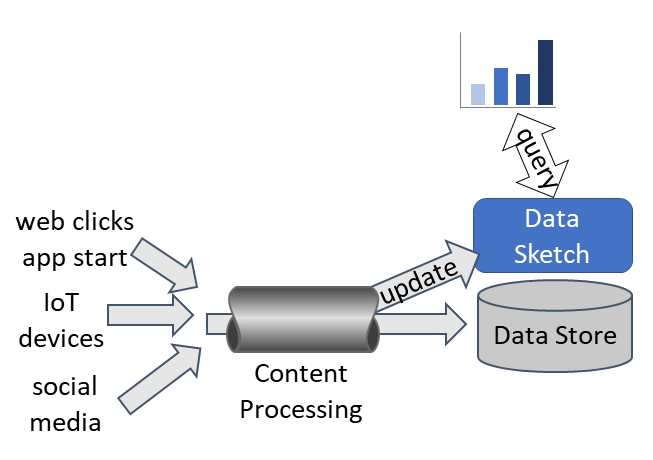
\includegraphics[height=1.6in]{graphics/fast-concurrent/pipeline-crop.png}
  \caption{Stream processing pipeline with data sketch.}
  \label{fc-fig:pipeline}
  \end{subfigure}
  \begin{subfigure}[b]{.55\linewidth}
    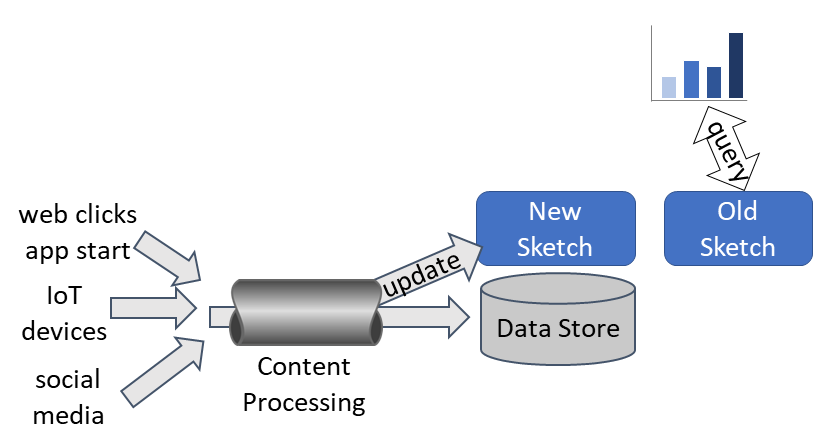
\includegraphics[height=1.6in]{graphics/fast-concurrent/epochs-crop.png}
  \caption{Using sketches in epochs.}
  \label{fc-fig:epochs}
  \end{subfigure}
\end{figure}

A sketch data structure is essentially a succinct (sublinear) summary of a stream that approximates a specific query, for instance, unique element count, quantile values, or frequent items. 
The approximation is typically very accurate -- the error drops fast with the stream size~\cite{Cormode:2017}. 

% Sketches today are sequential
Practical sketch implementations have recently emerged in toolkits~\cite{DataSketches}
and data analytics platforms (e.g., PowerDrill~\cite{heule2013hyperloglog}, Druid~\cite{druid}, 
Hillview~\cite{hillview}, and Presto~\cite{PrestoHLL}). 
However, these implementations are not thread-safe, allowing neither
parallel data ingestion nor concurrent queries and updates; concurrent use is prone to exceptions and 
gross estimation errors. Applications using these libraries are therefore required to explicitly protect all sketch API calls by locks~\cite{lee-groups-post, lee-issue}.
As a consequence of this limitation, typical deployments create sketches in epochs, where queries are referred to the sketch created in the previous epoch while new stream elements are directed to a new sketch, as illustrated in Figure~\ref{fc-fig:epochs}. This practice leads to stale query results and thus
loses the real-time quality of the system.  

\paragraph{Our approach.}
We present a generic approach to parallelizing data sketches efficiently while bounding the error that such a parallel implementation might induce. Our goal is to enable simultaneous queries and updates to the same sketch from multiple threads. Our solution is carefully designed to do so without slowing down operations as a result of synchronization.
This is particularly challenging because sketch libraries are extremely fast, often processing tens of millions of updates per second. 

We capitalize on the well-known sketch \emph{mergeability} property~\cite{Cormode:2017}, which enables computing a sketch 
over a stream by merging sketches over sub-streams. Previous works have exploited this property for distributed 
stream processing (e.g.,~\cite{heule2013hyperloglog, cormode2011algorithms}), devising solutions with a sequential bottleneck at the merge phase and where queries cannot
be served before all updates complete. 
In contrast, our method is based on shared memory and constantly propagates results to a queryable sketch.
Our solution architecture is illustrated in Figure~\ref{fc-fig:arch}. Multiple worker thread buffer updates in local sketches and periodically merge them into a global sketch; queries access the latter. 

\begin{figure}[htb]
  \begin{center}
    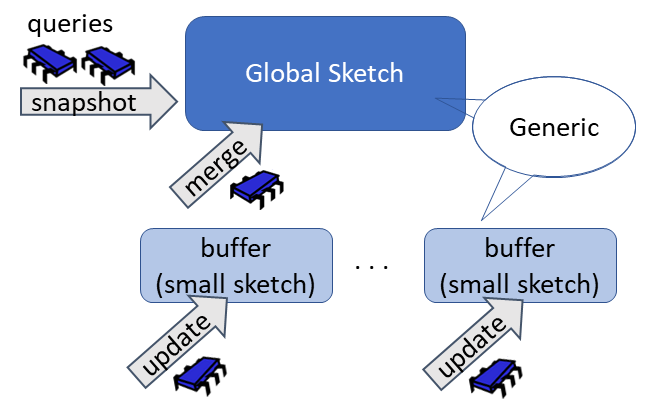
\includegraphics[width=0.5\textwidth]{graphics/fast-concurrent/arch-crop.png}
  \end{center}
  \caption{Concurrent sketches architecture.}
  \label{fc-fig:arch}
\end{figure}


We adaptively parallelize  stream processing:  
for small streams, we forgo parallel ingestion as it might introduce significant errors;  
but as the stream becomes large, we process it in parallel using small
thread-local sketches with continuous background propagation of local results to the common (queryable) sketch.

We instantiate our generic algorithm with a KMV $\Theta$ sketch~\cite{KMV},
which estimates the number of unique elements in a stream; a popular sketch
from the open-source Apache DataSketches library~\cite{DataSketches}.
We have contributed our implementation back to the Apache DataSketches 
library~\cite{ConcurrentThetaImp}. 
Yet we emphasize that our design is generic and applicable to additional sketches. 
We briefly discuss the applicability of our algorithm to additional popular sketches, such as Quantiles, CountMin, and HyperLogLog, 
where we discuss the generic algorithm (cf.~Section~\ref{fc-sec:genericAlg}).

Figure~\ref{fc-fig:performance} compares
the ingestion throughput of our concurrent $\Theta$ sketch to that of a lock-protected sequential sketch,
on multi-core hardware. As expected, the trivial solution does not scale whereas our algorithm scales linearly. 


\begin{figure}[htb]
  \begin{center}
    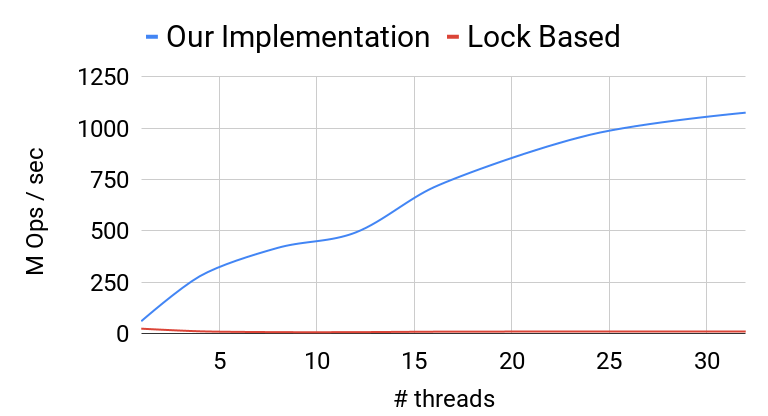
\includegraphics[width=0.6\textwidth]{graphics/fast-concurrent/concurrentThetaGraph.png}
  \end{center}
  \caption{Scalability of DataSketches' $\Theta$ sketch 
   protected by a lock vs.\ our concurrent implementation.}
  \label{fc-fig:performance}
\end{figure}

\paragraph{Error analysis.}
Concurrency might induce an error, and one of the main challenges we address is analyzing this error.
To begin with, our concurrent sketch is a concurrent data structure, and 
we need to specify its  semantics. We do so using a flavor of 
%\emph{relaxed consistency} due to Henzinger et al.~\cite{Henzinger}    
\emph{relaxed consistency} similar to~\cite{Henzinger, alistarh2018distributionally, talmage2014improving}    %specifically, a restricted form of their   \emph{out-of-order} relaxation 
that allows operations to ``overtake'' some other operations.  
Thus, a query may return a result that reflects all but a bounded number of the updates
that precede it. 
While relaxed semantics were previously used for data structures such as stacks~\cite{Henzinger}
and priority queues~\cite{alistarh, rihani2014multiqueues}, we believe that they are a natural fit for data sketches. 
This is because sketches are typically used to summarize streams that  arise from multiple real-world sources  
and are collected over a network with variable delays, and so even if the sketch ensures strict semantics, 
queries might miss some real-world events that occur before them. Additionally, sketches are inherently approximate.
Relaxing their semantics therefore ``makes sense'', as long as it does not excessively increase the expected error.
%Add that the error is addative and not multplicative
If a stream is much longer than the relaxation bound, then indeed the error induced by the relaxation is negligible. For instance, in a stream consisting of ten million events, missing a hundred (or even a thousand) of them will not make a big impact. 

Analytics platforms often use multiple sketches in order to capture different dimensions of the data. For instance, they may count the number of unique users from each region in a different sketch. 
Typically, a handful of popular sketches account for most events, and others are updated less frequently. Whereas the relaxation does not significantly affect the estimation in the popular sketches, since the error allowed by the relaxation is additive, in less popular sub-streams, it may have a large impact. 
This motivates our adaptive solution, which forgoes relaxing small streams altogether. 

% correctness roadmap: derandomise,  strong serialisability, Adversary model,

We show that under parallel ingestion, our algorithm satisfies relaxed consistency with a relaxation of up to $2Nb$, where $N$ is the number of worker threads and $b$ is the buffer size of each worker.  
In our example use case, $N$ is $12$ and $b$ ranges between $1$ and $5$. 

% But this raises a new difficulty: 
The proof involves some technical challenges. First, relaxed consistency is defined with regards to a deterministic specification, whereas sketches are randomized.
We therefore first de-randomize the sketch's behavior
by delegating the random coin flips to an oracle. We can then relax the resulting sequential specification.
Next, because our concurrent sketch is used within randomized algorithms, 
it is not enough to prove its linearizability. Rather, 
we prove that our generic concurrent algorithm instantiated with sequential sketch $S$
satisfies \emph{strong linearizability}~\cite{Wojciech} with regards to a relaxed sequential specification of the de-randomized $S$. We note, however, that supporting strong linearizability
did not incur additional costs nor did it impact the relaxation; we were able to prove that our original design was strongly linearizable. 

We then analyze the error for two types of relaxed sketches under random coin flips, with an adversarial scheduler that may delay operations in a way that maximizes the error. First, we consider the $\Theta$ sketch. For this sketch, its relative standard error has been analyzed, and we
show  that our concurrent implementation's error is coarsely bounded by twice
that of the corresponding sequential sketch. Second, we consider a family of \emph{probably approximately correct (PAC)}
sketches -- these are sketches that estimate some quantity with an error of at most $\epsilon$ with a probability of at least $1-\delta$. 
For an arbitrary PAC sketch estimating quantiles or counting unique elements, we show that the error induced by its relaxation approaches that of the original, non-relaxed sketch as the stream size tends to infinity.

\paragraph{Main contribution.} In summary, this paper tackles the problem of concurrent sketches,
offers a general efficient solution for it, and rigorously analyses this solution. While the
paper makes use of many known techniques, it combines them in a novel way.
The main technical challenges we address are (1) devising a high-performance generic algorithm 
that supports real-time queries concurrently with updates without inducing an excessive error; 
(2) proving the relaxed consistency of the algorithm; 
and (3) bounding the error induced by the relaxation in both short and long streams.

The paper proceeds as follows:
Section~\ref{fc-sec:model} lays out the model for our work and Section~\ref{fc-sec:background} provides background
on sequential sketches. In Section~\ref{fc-sec:concurrentSketches} we formulate a flavor of relaxed semantics
appropriate for data sketches. Section~\ref{fc-sec:genericAlg} presents our generic algorithm, and Section~\ref{fc-sec:proofs}
proves strong linearizability of our generic algorithm. Section~\ref{fc-sec:error-bounds} analyses
error bounds for example sketches. Section~\ref{fc-sec:eval} empirically studies the $\Theta$ sketch's performance
and error with different stream sizes. Finally, Section~\ref{fc-sec:discussion}
concludes.